\documentclass[twocolumn, a4j, 9pt, fleqn]{ltjsarticle}
\usepackage{enumitem}
\usepackage{url}
\usepackage{amsmath}
\usepackage[margin=10truemm]{geometry}
\usepackage{graphicx}
\usepackage{caption}
\captionsetup[figure]{format=plain, labelformat=simple, labelsep=period}

\setlength{\columnseprule}{0.1pt}
\setlength{\mathindent}{0pt}
\renewcommand{\baselinestretch}{0.8}
\renewcommand{\figurename}{Fig}
\setlength{\textfloatsep}{0pt}

\begin{document}

\title{Neural Network Input Features}
\author{93nezyr}
\maketitle

\section{入力特徴量生成・抽出}

ジョブショップスケジューリング問題(JSSP)における、特徴量選択方法について議論する。今回のJSSPは、ガントチャートで表現されるものとする。ガントチャートの行方向をJSSPにおけるリソース(マシン)、列方向をスケジューリングの時刻とすると、JSSPの状態には以下の変数が含まれる。

\begin{description}[style=multiline, leftmargin=10em]
  \item[$t$] スケジューリング中の現在時刻
  \item[$R$] リソースの集合
  \item[$R_i \in R$] リソース$i$
  \item[$J$] ジョブの集合
  \item[$J_j \in J$] ジョブ$j$
  \item[$O_m$] オペレーション$m$
  \item[$ON_{j}$] ジョブ$j$に含まれるオペレーション数
  \item[$OAR_{jm} = \{r \in R\}$] ジョブ$j$のオペレーション$m$が利用可能なリソースの集合
  \item[$PT_{ijm}$] ジョブ$j$のオペレーション$m$がリソース$i$で実行される場合の処理時間
  \item[$OR_{jm} \in R$] ジョブ$j$のオペレーション$m$が割り当てられているリソース
\end{description}

今回議論する問題では、必ず$OAR_{jm}$は一意に決まっており、各ジョブの各オペレーションが実行されるリソースは事前に決まっているとする。

\vskip\baselineskip
\subsection[1.2]{ディスパッチルール選択型モデル}

\cite{shuluo2020}では、下記の要素が状態から得られる特徴量として挙げられていた。

\begin{description}[style=multiline, leftmargin=10em]
  \item[$U_{ave}$] マシン$k$の稼働率を$U_k$としたときの、全マシンの$U_k$の平均値
  \item[$U_{std}$] 全マシンの$U_k$の標準偏差
  \item[$CRO_{ave}$] 全ジョブの操作終了数の平均値
  \item[$CRJ_{ave}$] 全ジョブの操作終了割合の平均値
  \item[$CRJ_{std}$] 全ジョブの操作終了割合の標準偏差
\end{description}

\noindent
残り2つの特徴量は、今回議論したい問題の場合、常に$0$となるので割愛する。
上記特徴量は、マシン・ジョブの区別がつかない特徴量なので、スケジューリング中の状態の変化に鈍感な箇所が存在する。上記特徴量に加えて以下の特徴量を追加する。

\begin{description}[style=multiline, leftmargin=10em]
  \item[$Type_{M_m}$] マシンのタイプ$m$
\end{description}

\begin{description}[style=multiline, leftmargin=15em]
  \item[$\bar{U_{k}} (Type_{M_k} = Type_{M_m})$] マシンタイプごとの$U_k$の平均値
  \item[$CPOC_j$] ジョブ$J_j$の終了した操作$PT_{ijm}$の操作時間の合計
  \item[$CPOR_j$] ジョブ$J_j$の未終了の操作$PT_{ijm}$の操作時間の合計
\end{description}

ただし、$CPOC_j$や$CPOR_j$をそのまま状態の特徴量として用いる場合、問題として設定されているジョブ数$|J|$によって特徴量の次元が変わってしまう。特徴量の次元を問題設定が変わっても固定のサイズにするために、以下のような工夫を導入する。

まず、\cite{shuluo2020}のような手法でJSSPを解く場合、ディスパッチルールから得られる解空間に限定されるため、$CPOR_j$は$h_m$と$w_m$をパラメータとして表現できるグラフに限定できる。

\begin{figure}
  \centering
  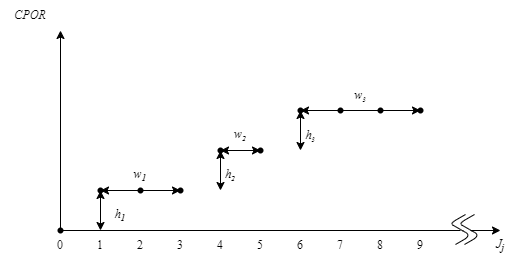
\includegraphics[width=\linewidth]{nninputfeatures01.png}
  \caption{$J$が全て同じオペレーションで構成されていた場合の$CPOR$グラフ}
  \label{fig:cpor}
\end{figure}
\newpage
Fig\ref{fig:cpor}のように、全てのジョブの$CPOR_j$を表現することで、解空間がディスパッチルールによって限定されている場合は、$h_m$と$w_m$だけで、全てのジョブの$CPOR_j$を再計算することが可能になる。
また、スケジュールの短中期的な予測に重要なのは、$h_m$と$w_m$の若い番号で再計算可能なジョブに集中する。そのため、$h_w$と$w_m$をどこまで保持するかの$m$はハイパーパラメータとし、この手法を導入することで、状態から得られる特徴量の次元を固定長とする。

\begin{thebibliography}{99}
  \bibitem{chandrashekar2014} chandrashekar2014 \\
  \url{https://www.sciencedirect.com/science/article/abs/pii/S0045790613003066}

  \bibitem{shuluo2020} shuluo2020
\end{thebibliography}

\vskip\baselineskip
\section*{補足}

(1)もしかしてこうやって何か情報を書いて \\
式(N)に示すとか言うて:
% \begin{align}
%   y = f(x)
% \end{align}
\begin{flalign}
  &y = f(x) &
\end{flalign}

\begin{flalign}
  &f(x) = \left\{
    \begin{array}{ll}
    1 & (x \geq 0)\\
    0 & (x < 0)
    \end{array}
    \right. &
\end{flalign}

\begin{align}
  y = &f(x) \\
  &f(x) = x^2
\end{align}

\end{document}
